\vspace*{4cm}
\part{Messresultate Mesh Benchmark}\label{part:MessresultateMeshBenchmark}
\vspace*{\fill}
\clearpage

\section{Messresultate}\label{sec:Messresultate}
Bei der Durchführung der Messungen innerhalb des Mesh Benchmarks wurde für jede Messung unter den entsprechenden Bedingungen, die in der Tabelle \ref{tab:MessungenMeshBenchmark} nochmals zusammengefasst sind, ein Messprotokoll resp. eine Auswertung erstellt. Diese detaillierten Auswertungen wurden im Anhang \ref{app:MessprotokolleMeshBenchmark} dem Bericht angefügt.



\todo[inline]{Cyrill}

\ref{app:Paper}

\todo[inline]{Verweis auf das Paper. Die wichtigsten Resultate und Erkenntnisse sind im Paper zusammengefasst.}

\subsection{Resultate}\label{subsec:Resultate}
\todo[inline]{Präsentation der Messresultate aus den Messungen der Mesh Netze. Als Grafiken inkl. beschreibendem Text. Keine Interpretation der Resultate. Vergleich der Resultate mit den verschiedenen Netzen.}

\todo[inline]{Verweis auf Messauswertungen im Anhang.}

\todo[inline]{Bild: Exemplarische Grafik z.B. Messung 1 Haus und Erläuterung wie die Messauswertungen zu lesen sind.}


\begin{table}[h]
\centering
\begin{tabular}{|c|c|c|c|c|c|} 
\hline
\textbf{\#}  & \textbf{Msg. Gen.}  & \textbf{Duration}  & \textbf{Msg. Cnt.}  & \textbf{Payload }  & \textbf{Disturbance}  \\ 
\hline
1 & Rand & 600s & 60 & Small & No \\ 
\hline
2 & Seq & 600s & 60 & Small & No \\ 
\hline
3 & Rand & 600s & 60 & Large & No \\ 
\hline
4 & Seq & 600s & 60 & Large & No \\ 
\hline
5 & Rand & 600s & 600 & Small & No \\ 
\hline
6 & Rand & 600s & 60 & Small & Yes \\ 
\hline
7 & Seq & 750s & 10 & Small & No \\ 
\hline
8 & Seq & 750s & 10 & Large & No \\
\hline
\end{tabular}
\caption{Messungen Mesh Benchmark}
\label{tab:MessungenMeshBenchmark}
\end{table}



\begin{figure}[h]
	\centering
	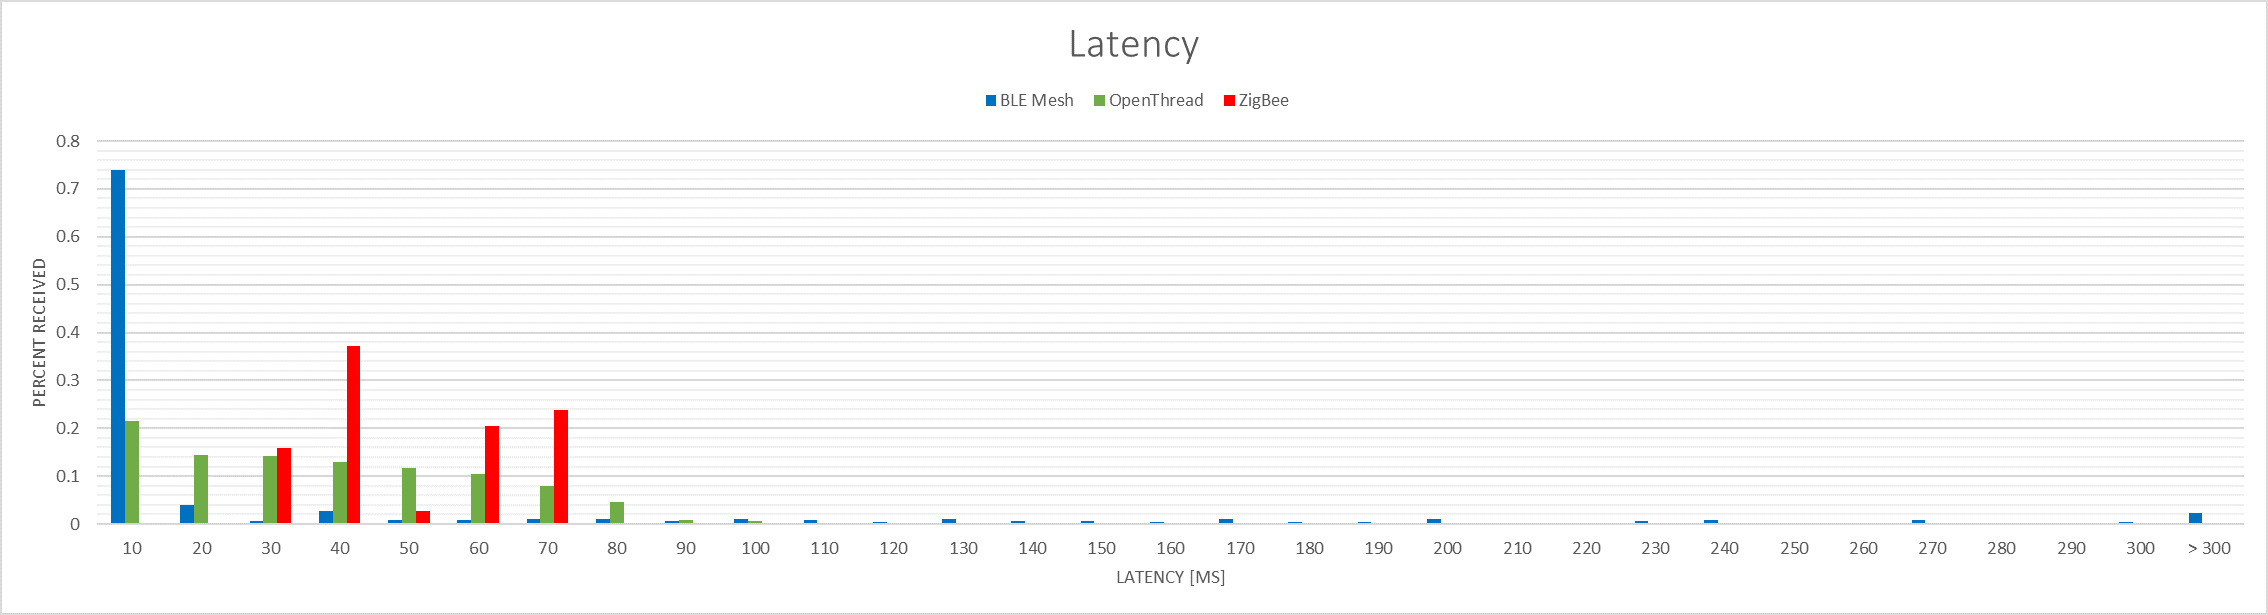
\includegraphics[width=\textwidth]{Latency_2_Wohnung.png}
	\caption{Verteilung der Latenzzeiten}
	\label{fig:VerteilungderLatenzzeiten}
\end{figure}


\begin{figure}[!htbp]
\centering
\begin{minipage}[b]{0.49\textwidth}
		\centering
		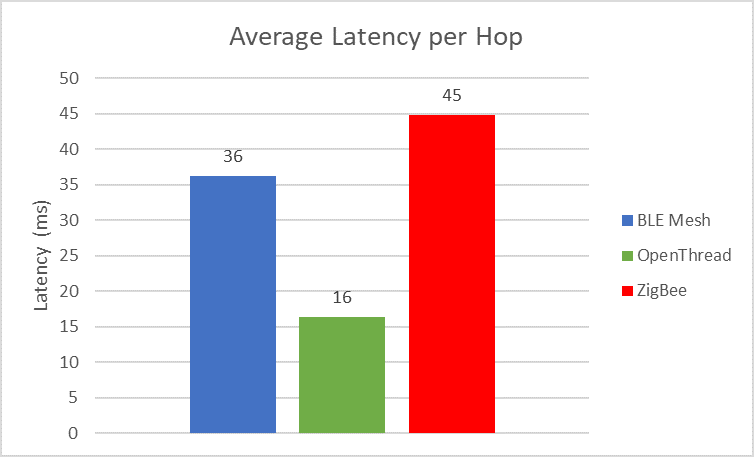
\includegraphics[width=\textwidth]{Average_Latency_per_Hop.png}
		\caption{Durchschnittliche Latenzzeit pro Hop}
		\label{fig:DurchschnittlicheLatenzzeit}
\end{minipage}
\begin{minipage}[b]{0.49\textwidth}
		\centering
		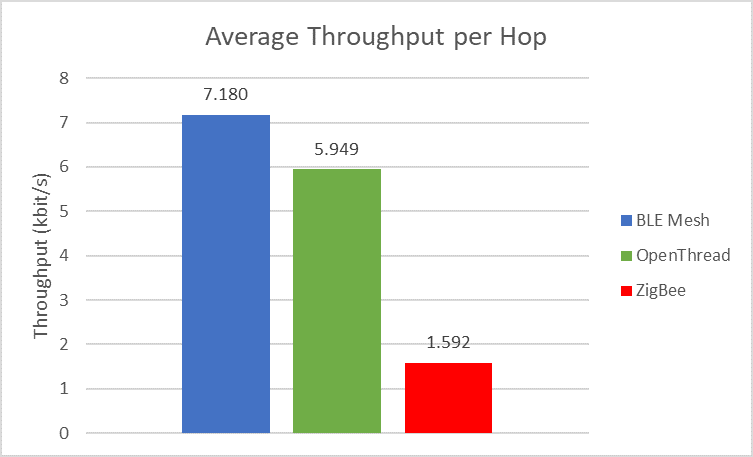
\includegraphics[width=\textwidth]{Average_Throughput_per_Hop.png}
		\caption{Durchschnittlicher Durchsatz pro Hop}
		\label{fig:DurchschnittlicherDurchsatz}
\end{minipage}
\end{figure}


\begin{figure}[!htbp]
\centering
\begin{minipage}[b]{0.49\textwidth}
		\centering
		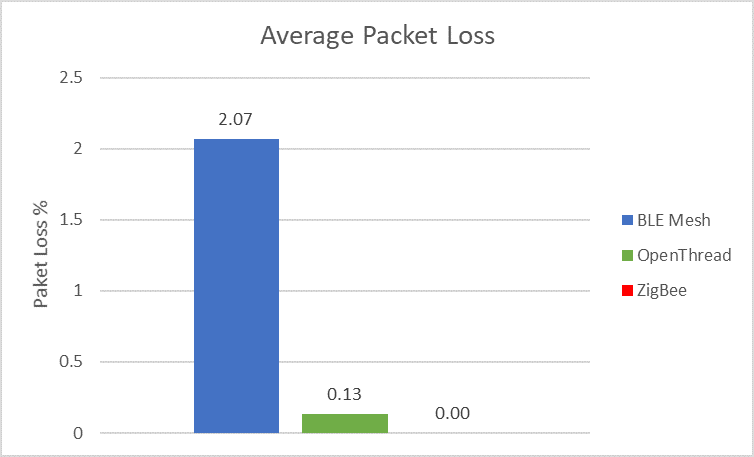
\includegraphics[width=\textwidth]{Average_Packet_Loss.png}
		\caption{Durchschnittlicher Paketverlust}
		\label{fig:DurchschnittlicherPaketverlust}
\end{minipage}
\begin{minipage}[b]{0.49\textwidth}
		\centering
		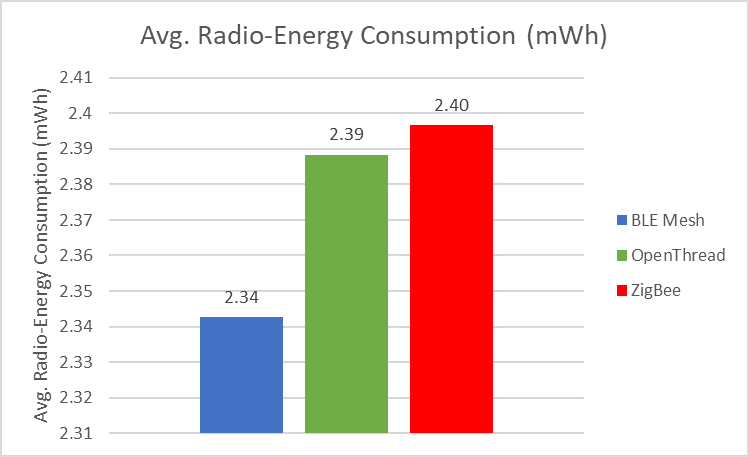
\includegraphics[width=\textwidth]{Average_Radio_Energy_Consumption.png}
		\caption{Durchschnittlicher Energieverbrauch}
		\label{fig:DurchschnittlicherEnergieverbrauch}
\end{minipage}
\end{figure}


\subsection{Validierung}\label{subsec:Validierung}

\todo[inline]{Überprüfung des eigenen Vorgehen usw.}

\subsection{Verifizierung}\label{subsec:Verifizierung}

\todo[inline]{Silabs Bericht}




